\renewcommand{\thefootnote}{\fnsymbol{footnote}}

\chapter[Introduction to exchange economies]%
 {Introduction to exchange economies}%
\label{ch:L6}

% 3) Reset things so later footnotes go back to 1, 2, 3, …
%\setcounter{footnote}{0}
\renewcommand{\thefootnote}{\arabic{footnote}}

\section{A primer on consumer choice}\label{sec:L6-cons}

Before we turn to general equilibrium, we need to review a few basic concepts about consumer choice. The setting is intuitive. There is a single individual \( i \) who consumes bundles of \( \ell \) different goods. The quantity of each good is represented by a real number. The consumption space is therefore \( \mathbb{R}^{\ell}_{+} \). A generic consumption bundle for individual \( i \) is \( x_i = (x_i^{1}, \dots, x_i^{\ell}) \). We use subscripts for individuals and superscripts for goods. For example, if \( \ell = 2 \), a consumption bundle could be \( x_i = (3,5) \), meaning 3 units of good 1 and 5 units of good 2, as represented in Figure~\ref{fig:L6-cons-bundle}. We index consumption bundles by \( i \) because later we will consider multiple individuals, each with their own consumption bundle.

\begin{figure}[H]
    \begin{center}
        \begin{tikzpicture}[x=0.70pt,y=0.70pt,yscale=-1,xscale=1]
            %uncomment if require: \path (0,385); %set diagram left start at 0, and has height of 385

            %Shape: Axis 2D [id:dp11721225431880233] 
            \draw  (135,317.12) -- (483,317.12)(169.8,23) -- (169.8,349.8) (476,312.12) -- (483,317.12) -- (476,322.12) (164.8,30) -- (169.8,23) -- (174.8,30)  ;
            %Shape: Circle [id:dp8937450517881602] 
            \draw  [fill={rgb, 255:red, 0; green, 0; blue, 0 }  ,fill opacity=1 ] (286.4,117.6) .. controls (286.4,115.94) and (287.74,114.6) .. (289.4,114.6) .. controls (291.06,114.6) and (292.4,115.94) .. (292.4,117.6) .. controls (292.4,119.26) and (291.06,120.6) .. (289.4,120.6) .. controls (287.74,120.6) and (286.4,119.26) .. (286.4,117.6) -- cycle ;
            %Straight Lines [id:da41961426078046393] 
            \draw  [dash pattern={on 4.5pt off 4.5pt}]  (289.4,117.6) -- (290,317.6) ;
            %Straight Lines [id:da9291508071819727] 
            \draw  [dash pattern={on 4.5pt off 4.5pt}]  (170,116.6) -- (289.4,117.6) ;

            % Text Node
            \draw (473,329.4) node [anchor=north west][inner sep=0.75pt]    {$x^{1}$};
            % Text Node
            \draw (130,17.4) node [anchor=north west][inner sep=0.75pt]    {$x^{2}$};
            % Text Node
            \draw (285,321.4) node [anchor=north west][inner sep=0.75pt]    {$3$};
            % Text Node
            \draw (154,110.4) node [anchor=north west][inner sep=0.75pt]    {$5$};
        \end{tikzpicture}
        \caption{A consumption bundle \( x_i = (3,5) \) in a two-good consumption space.}
        \label{fig:L6-cons-bundle}
    \end{center}
\end{figure}

Now suppose there is a vector of prices \( p = (p^{1}, \dots, p^{\ell}) \), where \( p^{k} \) is the price of good \( k \). Also assume that the individual has monetary wealth \( w_i \in \mathbb{R}_{+} \). He can therefore consume any bundle \( x_i \) such that total expenditure does not exceed \( w_i \), that is, such that \( p \cdot x_i \leq w_i \).\footnote{The operation \( \cdot \) denotes the product \( p^{1} x_i^{1} + \dots + p^{\ell} x_i^{\ell} \).} The set of all consumption bundles that satisfy this condition is called the \textbf{budget set}, and is denoted by

\[
    B(p,w_i) = \{ x_i \in \mathbb{R}^{\ell}_{+} \mid p \cdot x_i \leq w_i \}.
\]

The budget set is illustrated in Figure~\ref{fig:L6-cons-budget} in the two-good case. The budget line is the boundary of the budget set: it consists of all consumption bundles \( x_i \) such that \( p \cdot x_i = w_i \). If the individual consumes only good 1, then setting \( x_i^{2} = 0 \) yields \( x_i^{1} = \frac{w_i}{p^{1}} \). Similarly, if he consumes only good 2, then setting \( x_i^{1} = 0 \) yields \( x_i^{2} = \frac{w_i}{p^{2}} \). These two points are the intercepts of the budget line. The slope of the budget line is the relative price

\[
    w_i = p^{1} x_i^{1} + p^{2} x_i^{2} \implies x_i^{2} = \frac{w_i}{p^{2}} - \frac{p^{1}}{p^{2}} x_i^{1}.
\]


\begin{figure}[H]
    \begin{center}

        \tikzset{
            pattern size/.store in=\mcSize,
            pattern size = 5pt,
            pattern thickness/.store in=\mcThickness,
            pattern thickness = 0.3pt,
            pattern radius/.store in=\mcRadius,
            pattern radius = 1pt}
        \makeatletter
        \pgfutil@ifundefined{pgf@pattern@name@_g2kw7wjg6}{
            \pgfdeclarepatternformonly[\mcThickness,\mcSize]{_g2kw7wjg6}
            {\pgfqpoint{0pt}{0pt}}
            {\pgfpoint{\mcSize+\mcThickness}{\mcSize+\mcThickness}}
            {\pgfpoint{\mcSize}{\mcSize}}
            {
                \pgfsetcolor{\tikz@pattern@color}
                \pgfsetlinewidth{\mcThickness}
                \pgfpathmoveto{\pgfqpoint{0pt}{0pt}}
                \pgfpathlineto{\pgfpoint{\mcSize+\mcThickness}{\mcSize+\mcThickness}}
                \pgfusepath{stroke}
            }}
        \makeatother
        \tikzset{every picture/.style={line width=0.75pt}} %set default line width to 0.75pt        

        \begin{tikzpicture}[x=0.70pt,y=0.70pt,yscale=-1,xscale=1]
            %uncomment if require: \path (0,371); %set diagram left start at 0, and has height of 371

            %Shape: Axis 2D [id:dp08743181951332801] 
            \draw  (154,318.12) -- (502,318.12)(188.8,24) -- (188.8,350.8) (495,313.12) -- (502,318.12) -- (495,323.12) (183.8,31) -- (188.8,24) -- (193.8,31)  ;
            %Straight Lines [id:da35372055325342744] 
            \draw    (189,119.2) -- (376,318.2) ;
            %Shape: Arc [id:dp5558282393767194] 
            \draw  [draw opacity=0] (350.02,317.45) .. controls (350.01,317.2) and (350,316.95) .. (350,316.7) .. controls (350,310.25) and (355.18,304.87) .. (362.06,303.66) -- (365,316.7) -- cycle ; \draw   (350.02,317.45) .. controls (350.01,317.2) and (350,316.95) .. (350,316.7) .. controls (350,310.25) and (355.18,304.87) .. (362.06,303.66) ;
            %Straight Lines [id:da043045691510942063] 
            \draw    (353,251) -- (368.4,299.69) ;
            \draw [shift={(369,301.6)}, rotate = 252.45] [color={rgb, 255:red, 0; green, 0; blue, 0 }  ][line width=0.75]    (10.93,-3.29) .. controls (6.95,-1.4) and (3.31,-0.3) .. (0,0) .. controls (3.31,0.3) and (6.95,1.4) .. (10.93,3.29)   ;
            %Shape: Right Triangle [id:dp8729232973445785] 
            \draw  [pattern=_g2kw7wjg6,pattern size=15pt,pattern thickness=0.75pt,pattern radius=0pt, pattern color={rgb, 255:red, 0; green, 0; blue, 0}] (189,119.2) -- (376,318.2) -- (189,318.2) -- cycle ;

            % Text Node
            \draw (492,330.4) node [anchor=north west][inner sep=0.75pt]    {$x^{1}$};
            % Text Node
            \draw (149,18.4) node [anchor=north west][inner sep=0.75pt]    {$x^{2}$};
            % Text Node
            \draw (364,322.4) node [anchor=north west][inner sep=0.75pt]    {$\frac{w_{i}}{p^{1}}$};
            % Text Node
            \draw (159,99.4) node [anchor=north west][inner sep=0.75pt]    {$\frac{w_{i}}{p^{2}}$};
            % Text Node
            \draw (330,198.4) node [anchor=north west][inner sep=0.75pt]    {$-\frac{p^{1}}{p^{2}}$};
        \end{tikzpicture}
        \caption{A budget set \( B (p,w_i) \) in a two-good consumption space.}
        \label{fig:L6-cons-budget}
    \end{center}
\end{figure}

The individual has preferences over consumption bundles. In previous lectures we studied choice under uncertainty, where the outcome of a choice is to some extent random. Here there is no uncertainty: the individual has preferences \( \succsim_i \) over the consumption space \( \mathbb{R}^{\ell}_{+} \). As we did for the simplex, we can visualize these preferences by drawing indifference curves in the consumption space, as in Figure~\ref{fig:ind-curve}. All bundles on the same indifference curve are equally good for the individual.

\begin{figure}[H]
    \begin{center}
        \tikzset{every picture/.style={line width=0.75pt}} %set default line width to 0.75pt        

        \begin{tikzpicture}[x=0.50pt,y=0.50pt,yscale=-1,xscale=1]
            %uncomment if require: \path (0,365); %set diagram left start at 0, and has height of 365

            %Shape: Axis 2D [id:dp6420191159915085] 
            \draw  (139,309.12) -- (487,309.12)(173.8,15) -- (173.8,341.8) (480,304.12) -- (487,309.12) -- (480,314.12) (168.8,22) -- (173.8,15) -- (178.8,22)  ;
            %Curve Lines [id:da016781654661147116] 
            \draw    (209,41.6) .. controls (201,197.6) and (295,293.6) .. (450,280.6) ;

            % Text Node
            \draw (477,321.4) node [anchor=north west][inner sep=0.75pt]    {$x^{1}$};
            % Text Node
            \draw (134,9.4) node [anchor=north west][inner sep=0.75pt]    {$x^{2}$};
            % Text Node
            \draw (468,267.4) node [anchor=north west][inner sep=0.75pt]    {$\succsim_{i}$};
        \end{tikzpicture}
        \caption{An indifference curve in the consumption space \( \mathbb{R}^2 \).}
        \label{fig:ind-curve}
    \end{center}
\end{figure}

The individual would like to choose the most preferred bundle among those he can afford. Affordability is determined by the budget, and therefore by prices and wealth. Any most preferred affordable bundle is what the individual \textquote{demands} at the given prices and wealth. The \textbf{Walrasian demand} of an individual with preferences \( \succsim_i \), at prices \( p \) and wealth \( w_i \), is

\[
    D_i(p,w_i) = \{ x_i \in B(p,w_i) \mid x_i \succsim_i x_i' \ \text{for all} \ x_i' \in B(p,w_i) \}.
\]

In other words, a bundle \( x_i \) belongs to \( D_i(p,w_i) \) if it is affordable and at least as good as every other affordable bundle. In general, Walrasian demand is a set: it may happen that several affordable bundles tie for being best. We can visualize Walrasian demand graphically. For example, for the preferences represented in Figure~\ref{fig:ind-curve}, and assuming preferences are increasing in each good, Walrasian demand is a single point, as shown in Figure~\ref{fig:walrdem}.

\begin{figure}[H]
    \begin{center}
        \tikzset{every picture/.style={line width=0.75pt}} %set default line width to 0.75pt        

        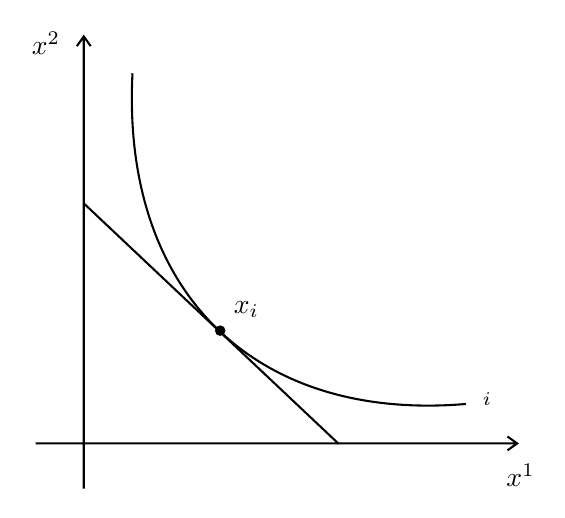
\begin{tikzpicture}[x=0.50pt,y=0.50pt,yscale=-1,xscale=1]
            %uncomment if require: \path (0,372); %set diagram left start at 0, and has height of 372

            %Shape: Axis 2D [id:dp46449684109220557] 
            \draw  (142,316.12) -- (490,316.12)(176.8,22) -- (176.8,348.8) (483,311.12) -- (490,316.12) -- (483,321.12) (171.8,29) -- (176.8,22) -- (181.8,29)  ;
            %Curve Lines [id:da501816174600593] 
            \draw    (212,48.6) .. controls (204,204.6) and (298,300.6) .. (453,287.6) ;
            %Straight Lines [id:da6392200784677712] 
            \draw    (177,142.8) -- (361,316.4) ;
            %Shape: Circle [id:dp48927821171680974] 
            \draw  [fill={rgb, 255:red, 0; green, 0; blue, 0 }  ,fill opacity=1 ] (272.4,234.6) .. controls (272.4,232.94) and (273.74,231.6) .. (275.4,231.6) .. controls (277.06,231.6) and (278.4,232.94) .. (278.4,234.6) .. controls (278.4,236.26) and (277.06,237.6) .. (275.4,237.6) .. controls (273.74,237.6) and (272.4,236.26) .. (272.4,234.6) -- cycle ;

            % Text Node
            \draw (480,328.4) node [anchor=north west][inner sep=0.75pt]    {$x^{1}$};
            % Text Node
            \draw (137,16.4) node [anchor=north west][inner sep=0.75pt]    {$x^{2}$};
            % Text Node
            \draw (463,277.4) node [anchor=north west][inner sep=0.75pt]    {$\succsim _{i}$};
            % Text Node
            \draw (283,211.4) node [anchor=north west][inner sep=0.75pt]    {$x_{i}$};
        \end{tikzpicture}
        \caption{Walrasian demand for preferences \( \succsim_i \).}
        \label{fig:walrdem}
    \end{center}
\end{figure}

\begin{techremark}
    What kind of indifference curves should \( \succsim_i \) have for the Walrasian demand to contain more than one element? Can you construct an example in the graph?
\end{techremark}

In the next section, we build on these basics to consider the choices of two individuals simultaneously.

\section{Illustrative example of exchange economy}\label{sec:L6-example}

We now move from individual choice, which we studied in the previous lectures, to \textit{collective} choice. In general equilibrium theory, we generalize concepts from individual consumer choice to an economy with multiple individuals. In this section we start from a simple example with two individuals and two goods, which we will later generalize.

Suppose there are two individuals \( 1 \) and \( 2 \) and two goods. Each individual has the consumption space \( \mathbb{R}^{2}_{+} \), and a consumption bundle \( x_i = (x_i^{1}, x_i^{2}) \). We can represent the consumption space of individual \( 1 \), together with his indifference curves, as we did in Figure~\ref{fig:ind-curve}. For individual \( 2 \), we can do the same, but suppose we draw his consumption space upside down, as in Figure~\ref{fig:L6-ind-2} (bear with me).

\begin{figure}[H]
    \begin{center}
        \begin{tikzpicture}[x=0.65pt,y=0.65pt,yscale=-1,xscale=1]
            %uncomment if require: \path (0,405); %set diagram left start at 0, and has height of 405
            %Shape: Axis 2D [id:dp8034807906536237] 
            \draw  (498.91,55.56) -- (150.91,55.8)(464.31,349.7) -- (464.09,22.9) (157.91,60.8) -- (150.91,55.8) -- (157.91,50.8) (469.31,342.7) -- (464.31,349.7) -- (459.31,342.71)  ;

            % Text Node
            \draw (155,27.4) node [anchor=north west][inner sep=0.75pt]    {$x^{1}$};
            % Text Node
            \draw (477,331.4) node [anchor=north west][inner sep=0.75pt]    {$x^{2}$};
        \end{tikzpicture}
        \caption{Consumption space of individual 2 upside down.}
        \label{fig:L6-ind-2}
    \end{center}
\end{figure}

Now we can combine the two consumption spaces in a single graph, called the \textbf{Edgeworth box}, as in Figure~\ref{fig:L6-edgeworth-box}. The total width of the box is the total amount of good \( 1 \) available in the economy as a whole, and the total height is the total amount of good \( 2 \) available. The two origins \( O_1 \) and \( O_2 \) are at the bottom left and top right corners of the box, respectively. Each point in the box represents an \textbf{allocation} of goods between the two individuals. For example, the point \( x \) represents the allocation in which individual \( 1 \) consumes \( (x_1^{1}, x_1^{2}) \) and individual \( 2 \) consumes \( (x_2^{1}, x_2^{2}) \). The consumption of each individual \( i \) is read by viewing the box from the perspective of origin \( O_i \).

\begin{figure}[H]
    \begin{center}
        \begin{tikzpicture}[x=0.65pt,y=0.65pt,yscale=-1,xscale=1]
            %uncomment if require: \path (0,484); %set diagram left start at 0, and has height of 484

            %Shape: Axis 2D [id:dp40102790828068324] 
            \draw  (127,388.6) -- (489,388.6)(163.2,35.8) -- (163.2,427.8) (482,383.6) -- (489,388.6) -- (482,393.6) (158.2,42.8) -- (163.2,35.8) -- (168.2,42.8)  ;
            %Shape: Axis 2D [id:dp3759884204481627] 
            \draw  (497,69.9) -- (141,69.9)(461.4,421.8) -- (461.4,30.8) (148,74.9) -- (141,69.9) -- (148,64.9) (466.4,414.8) -- (461.4,421.8) -- (456.4,414.8)  ;
            %Shape: Circle [id:dp6709728610513666] 
            \draw  [fill={rgb, 255:red, 0; green, 0; blue, 0 }  ,fill opacity=1 ] (337.4,200.6) .. controls (337.4,198.94) and (338.74,197.6) .. (340.4,197.6) .. controls (342.06,197.6) and (343.4,198.94) .. (343.4,200.6) .. controls (343.4,202.26) and (342.06,203.6) .. (340.4,203.6) .. controls (338.74,203.6) and (337.4,202.26) .. (337.4,200.6) -- cycle ;

            % Text Node
            \draw (127,399.6) node [anchor=north west][inner sep=0.75pt]    {$O_{1}$};
            % Text Node
            \draw (474,40.6) node [anchor=north west][inner sep=0.75pt]    {$O_{2}$};
            % Text Node
            \draw (307,398) node [anchor=north west][inner sep=0.75pt]    {$x^{1}$};
            % Text Node
            \draw (134,220.4) node [anchor=north west][inner sep=0.75pt]    {$x^{2}$};
            % Text Node
            \draw (345,182.4) node [anchor=north west][inner sep=0.75pt]    {$x$};


        \end{tikzpicture}
        \caption{Edgeworth box representing the consumption spaces of individuals 1 and 2.}
        \label{fig:L6-edgeworth-box}
    \end{center}
\end{figure}

We can also represent the indifference curves of both individuals through \( x \) in the Edgeworth box, as in Figure~\ref{fig:L6-edgeworth-indiff}. The indifference curve of individual \( i \) is indicated with \( \succsim_i \).

\begin{figure}[H]
    \begin{center}
        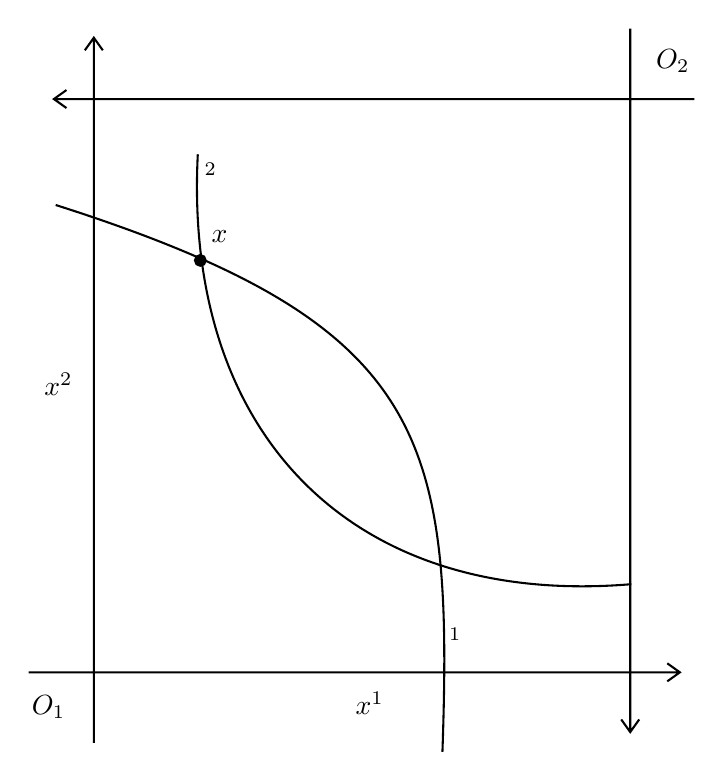
\begin{tikzpicture}[x=0.65pt,y=0.65pt,yscale=-1,xscale=1]
            %uncomment if require: \path (0,484); %set diagram left start at 0, and has height of 484
            %Shape: Axis 2D [id:dp40102790828068324] 
            \draw  (127,388.6) -- (489,388.6)(163.2,35.8) -- (163.2,427.8) (482,383.6) -- (489,388.6) -- (482,393.6) (158.2,42.8) -- (163.2,35.8) -- (168.2,42.8)  ;
            %Shape: Axis 2D [id:dp3759884204481627] 
            \draw  (497,69.9) -- (141,69.9)(461.4,421.8) -- (461.4,30.8) (148,74.9) -- (141,69.9) -- (148,64.9) (466.4,414.8) -- (461.4,421.8) -- (456.4,414.8)  ;
            %Shape: Circle [id:dp6709728610513666] 
            \draw  [fill={rgb, 255:red, 0; green, 0; blue, 0 }  ,fill opacity=1 ] (219.4,159.6) .. controls (219.4,157.94) and (220.74,156.6) .. (222.4,156.6) .. controls (224.06,156.6) and (225.4,157.94) .. (225.4,159.6) .. controls (225.4,161.26) and (224.06,162.6) .. (222.4,162.6) .. controls (220.74,162.6) and (219.4,161.26) .. (219.4,159.6) -- cycle ;
            %Curve Lines [id:da47481039339768105] 
            \draw    (221,100.6) .. controls (213,256.6) and (307,352.6) .. (462,339.6) ;
            %Curve Lines [id:da5885667761847703] 
            \draw    (142,128.8) .. controls (349,194.8) and (363,256.8) .. (357,432.8) ;

            % Text Node
            \draw (127,399.6) node [anchor=north west][inner sep=0.75pt]    {$O_{1}$};
            % Text Node
            \draw (474,40.6) node [anchor=north west][inner sep=0.75pt]    {$O_{2}$};
            % Text Node
            \draw (307,398) node [anchor=north west][inner sep=0.75pt]    {$x^{1}$};
            % Text Node
            \draw (134,220.4) node [anchor=north west][inner sep=0.75pt]    {$x^{2}$};
            % Text Node
            \draw (227,141.4) node [anchor=north west][inner sep=0.75pt]    {$x$};
            % Text Node
            \draw (359,362.4) node [anchor=north west][inner sep=0.75pt]    {$\succsim_{1}$};
            % Text Node
            \draw (223,104) node [anchor=north west][inner sep=0.75pt]    {$\succsim_{2}$};
        \end{tikzpicture}
        \caption{Edgeworth box representing the consumption spaces of individuals 1 and 2.}
        \label{fig:L6-edgeworth-indiff}
    \end{center}
\end{figure}

We assume that preferences are increasing in each good. Therefore, both individuals would like to move away from the origin of their own consumption space. For example, individual \( 1 \) prefers being on the dotted indifference curve rather than on the solid one in Figure~\ref{fig:L6-edgeworth-indiff}.

\begin{figure}[H]
    \begin{center}
        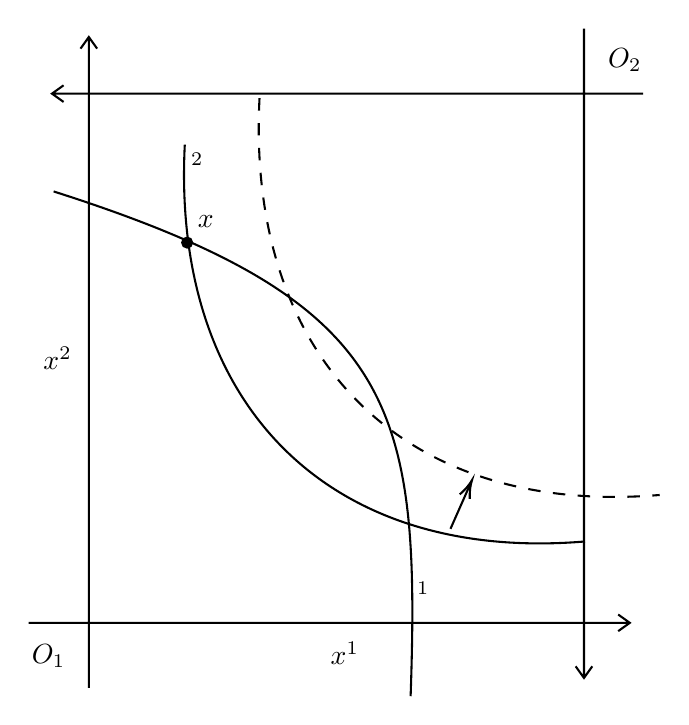
\begin{tikzpicture}[x=0.60pt,y=0.60pt,yscale=-1,xscale=1]
            %uncomment if require: \path (0,484); %set diagram left start at 0, and has height of 484

            %Shape: Axis 2D [id:dp40102790828068324] 
            \draw  (127,388.6) -- (489,388.6)(163.2,35.8) -- (163.2,427.8) (482,383.6) -- (489,388.6) -- (482,393.6) (158.2,42.8) -- (163.2,35.8) -- (168.2,42.8)  ;
            %Shape: Axis 2D [id:dp3759884204481627] 
            \draw  (497,69.9) -- (141,69.9)(461.4,421.8) -- (461.4,30.8) (148,74.9) -- (141,69.9) -- (148,64.9) (466.4,414.8) -- (461.4,421.8) -- (456.4,414.8)  ;
            %Shape: Circle [id:dp6709728610513666] 
            \draw  [fill={rgb, 255:red, 0; green, 0; blue, 0 }  ,fill opacity=1 ] (219.4,159.6) .. controls (219.4,157.94) and (220.74,156.6) .. (222.4,156.6) .. controls (224.06,156.6) and (225.4,157.94) .. (225.4,159.6) .. controls (225.4,161.26) and (224.06,162.6) .. (222.4,162.6) .. controls (220.74,162.6) and (219.4,161.26) .. (219.4,159.6) -- cycle ;
            %Curve Lines [id:da47481039339768105] 
            \draw    (221,100.6) .. controls (213,256.6) and (307,352.6) .. (462,339.6) ;
            %Curve Lines [id:da5885667761847703] 
            \draw    (142,128.8) .. controls (349,194.8) and (363,256.8) .. (357,432.8) ;
            %Curve Lines [id:da5975153383572774] 
            \draw  [dash pattern={on 4.5pt off 4.5pt}]  (266,72.6) .. controls (258,228.6) and (352,324.6) .. (507,311.6) ;
            %Straight Lines [id:da20949155455549462] 
            \draw    (381,332) -- (393.19,304.43) ;
            \draw [shift={(394,302.6)}, rotate = 113.85] [color={rgb, 255:red, 0; green, 0; blue, 0 }  ][line width=0.75]    (10.93,-3.29) .. controls (6.95,-1.4) and (3.31,-0.3) .. (0,0) .. controls (3.31,0.3) and (6.95,1.4) .. (10.93,3.29)   ;

            % Text Node
            \draw (127,399.6) node [anchor=north west][inner sep=0.75pt]    {$O_{1}$};
            % Text Node
            \draw (474,40.6) node [anchor=north west][inner sep=0.75pt]    {$O_{2}$};
            % Text Node
            \draw (307,398) node [anchor=north west][inner sep=0.75pt]    {$x^{1}$};
            % Text Node
            \draw (134,220.4) node [anchor=north west][inner sep=0.75pt]    {$x^{2}$};
            % Text Node
            \draw (227,141.4) node [anchor=north west][inner sep=0.75pt]    {$x$};
            % Text Node
            \draw (359,362.4) node [anchor=north west][inner sep=0.75pt]    {$\succsim_{1}$};
            % Text Node
            \draw (223,104) node [anchor=north west][inner sep=0.75pt]    {$\succsim_{2}$};
        \end{tikzpicture}
        \caption{Individual \( 1 \) would prefer to move on the dotted indifference curve.}
        \label{fig:L6-edgeworth-indiff1}
    \end{center}
\end{figure}

Now suppose that each individual has an initial endowment of goods, that is, a bundle of goods that he initially owns. The endowment of individual \( i \) is denoted by \( e_i = (e_i^{1}, e_i^{2}) \). The initial endowments determine the initial allocation in the Edgeworth box. The total endowment in the economy is \( e = e_1 + e_2 \), and this determines the size of the Edgeworth box. In principle, individuals can trade their endowments to reach preferred allocations.

Now suppose there are prices in the economy, given by the vector \( p = (p^{1}, p^{2}) \), one for each good. Given prices and endowments, we can compute the initial wealth of each individual. In individual consumer choice, wealth was given as a monetary amount \( w_i \), whereas here it is the value of the endowment at the given prices. The wealth of individual \( i \) is therefore \( w_i = p \cdot e_i = p^{1} e_i^{1} + p^{2} e_i^{2} \). Hence, the budget set of individual \( i \) consists of all consumption bundles \( x_i \) such that \( p \cdot x_i \leq p \cdot e_i \). So the budget set is\footnote{There is a slight abuse of notation: to be fully consistent with the earlier definition, I should write \( B(p, p \cdot e_i) \).}

\[
    B(p, e_i) = \{ x_i \in \mathbb{R}^{2}_{+} \mid p \cdot x_i \leq p \cdot e_i \}.
\]

We can draw the budget line in the Edgeworth box, as in Figure~\ref{fig:L6-edgeworth-budget}. First, it passes through the endowment point, since the individual can always afford to consume his initial endowment. Second, the slope of the budget line is given by the relative price, as we saw in individual consumer choice.


\begin{figure}[H]
    \begin{center}
        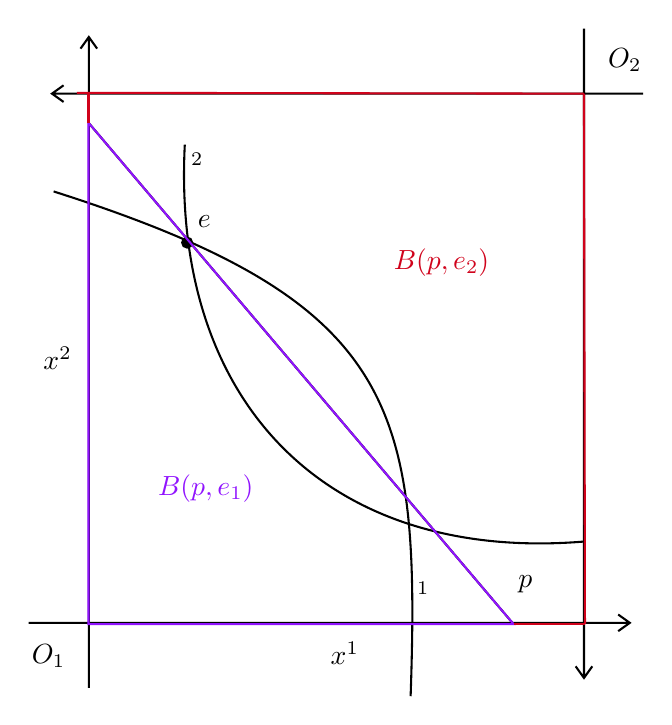
\begin{tikzpicture}[x=0.60pt,y=0.60pt,yscale=-1,xscale=1]
            %uncomment if require: \path (0,553); %set diagram left start at 0, and has height of 553

            %Shape: Axis 2D [id:dp2059171574689569] 
            \draw  (114,429.6) -- (476,429.6)(150.2,76.8) -- (150.2,468.8) (469,424.6) -- (476,429.6) -- (469,434.6) (145.2,83.8) -- (150.2,76.8) -- (155.2,83.8)  ;
            %Shape: Axis 2D [id:dp9098391304110112] 
            \draw  (484,110.9) -- (128,110.9)(448.4,462.8) -- (448.4,71.8) (135,115.9) -- (128,110.9) -- (135,105.9) (453.4,455.8) -- (448.4,462.8) -- (443.4,455.8)  ;
            %Shape: Circle [id:dp29037196470099513] 
            \draw  [fill={rgb, 255:red, 0; green, 0; blue, 0 }  ,fill opacity=1 ] (206.4,200.6) .. controls (206.4,198.94) and (207.74,197.6) .. (209.4,197.6) .. controls (211.06,197.6) and (212.4,198.94) .. (212.4,200.6) .. controls (212.4,202.26) and (211.06,203.6) .. (209.4,203.6) .. controls (207.74,203.6) and (206.4,202.26) .. (206.4,200.6) -- cycle ;
            %Curve Lines [id:da4738735984745992] 
            \draw    (208,141.6) .. controls (200,297.6) and (294,393.6) .. (449,380.6) ;
            %Curve Lines [id:da9965125080225232] 
            \draw    (129,169.8) .. controls (336,235.8) and (350,297.8) .. (344,473.8) ;
            %Straight Lines [id:da01912696996270169] 
            \draw    (150,128.4) -- (406,430.4) ;
            %Shape: Right Triangle [id:dp4353433944244913] 
            \draw  [color={rgb, 255:red, 144; green, 19; blue, 254 }  ,draw opacity=1 ] (150,128.4) -- (406,430.4) -- (150,430.4) -- cycle ;
            %Straight Lines [id:da12633324358064502] 
            \draw [color={rgb, 255:red, 208; green, 2; blue, 27 }  ,draw opacity=1 ]   (150,110.4) -- (150,128.4) ;
            %Straight Lines [id:da31044846939436144] 
            \draw [color={rgb, 255:red, 208; green, 2; blue, 27 }  ,draw opacity=1 ]   (143,110.4) -- (448.4,110.9) ;
            %Straight Lines [id:da5047439421029256] 
            \draw [color={rgb, 255:red, 208; green, 2; blue, 27 }  ,draw opacity=1 ]   (448.4,110.9) -- (449,430.4) ;
            %Straight Lines [id:da4524801166768464] 
            \draw [color={rgb, 255:red, 208; green, 2; blue, 27 }  ,draw opacity=1 ]   (406,430.4) -- (449,430.4) ;

            % Text Node
            \draw (114,440.6) node [anchor=north west][inner sep=0.75pt]    {$O_{1}$};
            % Text Node
            \draw (461,81.6) node [anchor=north west][inner sep=0.75pt]    {$O_{2}$};
            % Text Node
            \draw (294,439) node [anchor=north west][inner sep=0.75pt]    {$x^{1}$};
            % Text Node
            \draw (121,261.4) node [anchor=north west][inner sep=0.75pt]    {$x^{2}$};
            % Text Node
            \draw (214,182.4) node [anchor=north west][inner sep=0.75pt]    {$e$};
            % Text Node
            \draw (346,403.4) node [anchor=north west][inner sep=0.75pt]    {$\succsim_{1}$};
            % Text Node
            \draw (210,145) node [anchor=north west][inner sep=0.75pt]    {$\succsim_{2}$};
            % Text Node
            \draw (407,399.4) node [anchor=north west][inner sep=0.75pt]    {$p$};
            % Text Node
            \draw (190,338.4) node [anchor=north west][inner sep=0.75pt]  [color={rgb, 255:red, 144; green, 19; blue, 254 }  ,opacity=1 ]  {$B( p,e_{1})$};
            % Text Node
            \draw (332,202.4) node [anchor=north west][inner sep=0.75pt]  [color={rgb, 255:red, 208; green, 2; blue, 27 }  ,opacity=1 ]  {$B( p,e_{2})$};
        \end{tikzpicture}
        \caption{Budget line and budget sets in the Edgeworth box.}
        \label{fig:L6-edgeworth-budget}
    \end{center}
\end{figure}

Individuals may then choose their favourite consumption bundle in their budget set according to their preferences, that is, a bundle in their Walrasian demand set. When both individuals choose a bundle from their Walrasian demand set at the same prices, we can ask whether total demand is equal to the total endowment in the economy. If this is the case, we have found a \textbf{Walrasian equilibrium}, as illustrated in Figure~\ref{fig:L6-edgeworth-walr}.

\begin{figure}[H]
    \begin{center}
        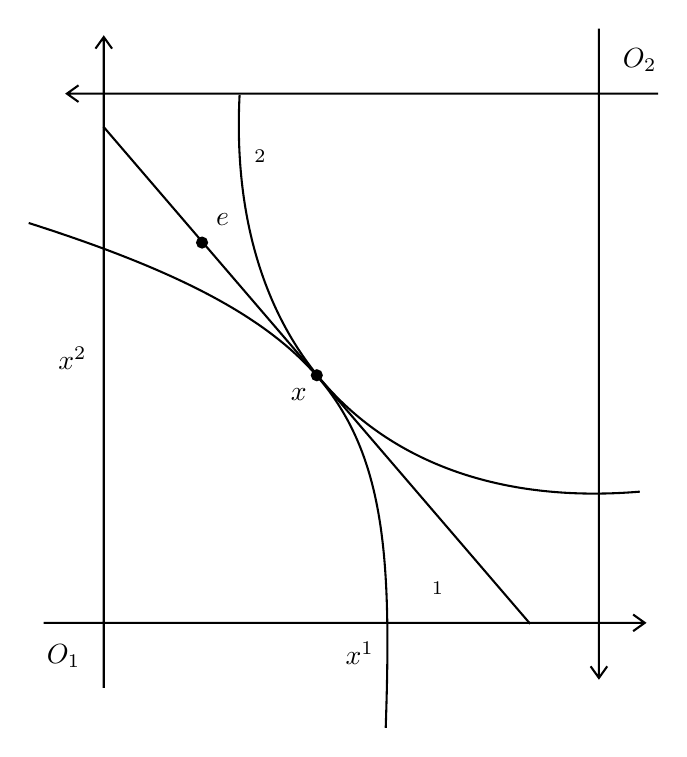
\begin{tikzpicture}[x=0.60pt,y=0.60pt,yscale=-1,xscale=1]
            %uncomment if require: \path (0,590); %set diagram left start at 0, and has height of 590

            %Shape: Axis 2D [id:dp0067678999696174635] 
            \draw  (124,450.8) -- (486,450.8)(160.2,98) -- (160.2,490) (479,445.8) -- (486,450.8) -- (479,455.8) (155.2,105) -- (160.2,98) -- (165.2,105)  ;
            %Shape: Axis 2D [id:dp7749821148951912] 
            \draw  (494,132.1) -- (138,132.1)(458.4,484) -- (458.4,93) (145,137.1) -- (138,132.1) -- (145,127.1) (463.4,477) -- (458.4,484) -- (453.4,477)  ;
            %Shape: Circle [id:dp8962890071231959] 
            \draw  [fill={rgb, 255:red, 0; green, 0; blue, 0 }  ,fill opacity=1 ] (216.4,221.8) .. controls (216.4,220.14) and (217.74,218.8) .. (219.4,218.8) .. controls (221.06,218.8) and (222.4,220.14) .. (222.4,221.8) .. controls (222.4,223.46) and (221.06,224.8) .. (219.4,224.8) .. controls (217.74,224.8) and (216.4,223.46) .. (216.4,221.8) -- cycle ;
            %Curve Lines [id:da8966169090103205] 
            \draw    (242,132.8) .. controls (234,288.8) and (328,384.8) .. (483,371.8) ;
            %Curve Lines [id:da0832517248134198] 
            \draw    (115,210) .. controls (322,276) and (336,338) .. (330,514) ;
            %Straight Lines [id:da6569099642091198] 
            \draw    (160,152) -- (417,451.4) ;
            %Shape: Circle [id:dp266854681951736] 
            \draw  [fill={rgb, 255:red, 0; green, 0; blue, 0 }  ,fill opacity=1 ] (285.5,301.7) .. controls (285.5,300.04) and (286.84,298.7) .. (288.5,298.7) .. controls (290.16,298.7) and (291.5,300.04) .. (291.5,301.7) .. controls (291.5,303.36) and (290.16,304.7) .. (288.5,304.7) .. controls (286.84,304.7) and (285.5,303.36) .. (285.5,301.7) -- cycle ;

            % Text Node
            \draw (124,461.8) node [anchor=north west][inner sep=0.75pt]    {$O_{1}$};
            % Text Node
            \draw (471,102.8) node [anchor=north west][inner sep=0.75pt]    {$O_{2}$};
            % Text Node
            \draw (304,460.2) node [anchor=north west][inner sep=0.75pt]    {$x^{1}$};
            % Text Node
            \draw (131,282.6) node [anchor=north west][inner sep=0.75pt]    {$x^{2}$};
            % Text Node
            \draw (226,202.6) node [anchor=north west][inner sep=0.75pt]    {$e$};
            % Text Node
            \draw (356,424.6) node [anchor=north west][inner sep=0.75pt]    {$\succsim_{1}$};
            % Text Node
            \draw (249,164.2) node [anchor=north west][inner sep=0.75pt]    {$\succsim_{2}$};
            % Text Node
            \draw (271,308) node [anchor=north west][inner sep=0.75pt]    {$x$};


        \end{tikzpicture}

        \caption{Walrasian equilibrium \( x \) in the Edgeworth box.}
        \label{fig:L6-edgeworth-walr}
    \end{center}
\end{figure}

In the rest of the lectures, we mainly focus on the properties of Walrasian equilibria. One might wonder whether Walrasian equilibria induce allocations that are desirable in some sense. Let us consider a possible criterion of desirability. Take an allocation \( x \) in the Edgeworth box. Is there any other allocation \( x' \) such that both individuals weakly prefer \( x' \) to \( x \), and at least one of them strictly prefers it? If such an allocation \( x' \) exists, then we say that \( x' \) is a \textbf{Pareto improvement} over \( x \), since at least one individual is strictly better off and no individual is worse off. If no such allocation \( x' \) exists, then we say that \( x \) is \textbf{Pareto optimal}. As an example, the endowment allocation \( e \) in Figure~\ref{fig:L6-edgeworth-walr} is \textbf{not} Pareto optimal. Pareto optimality is arguably a minimal requirement for an allocation to be considered desirable. The first theorem of welfare economics states that, under some assumptions, any Walrasian equilibrium allocation is Pareto optimal, and therefore that Walrasian equilibria satisfy this minimal requirement of desirability.\footnote{However, some people reject Pareto optimality. One reason is that it is defined entirely in terms of preferences, while we might want to evaluate allocations using other considerations.} In fact, the Walrasian equilibrium allocation \( x \) in Figure~\ref{fig:L6-edgeworth-walr} is Pareto optimal.

However, Pareto optimality is sometimes too weak. For example, the corners of the Edgeworth box are Pareto optimal, but one might argue that they are not desirable allocations. Pareto optimality is a requirement of \textit{efficiency}. No resource is wasted in achieving preference satisfaction. An efficiency requirement might be complemented by a \textit{fairness} requirement. Luckily, there is an extensive literature on fairness in social choice theory, deeply informed by philosophical work.\footnote{If you are interested, check \cite{moulinAxiomsCooperativeDecision1988}, \cite{youngEquityTheoryPractice1994}, \cite{roemerTheoriesDistributiveJustice1996}, \cite{moulinFairDivisionCollective2004}, \cite{fleurbaeyFairnessResponsibilityWelfare2008}, \cite{fleurbaeyTheoryFairnessSocial2011}, \cite{thomsonFairAllocationRules2011}. Gabriel Carroll has a syllabus for an interesting class \href{https://www.economics.utoronto.ca/gabriel.carroll/317syllabus-win24.pdf}{here}, if you want to explore further.}

A notion of fairness that has been widely studied is that of \textbf{envy-freeness}.\footnote{Apparently it has been introduced by Jan Tinbergen \citep{heilmannNoEnvyJan2021}.} An allocation \( x \) is envy-free if no individual prefers another individual's bundle to his own. In other words, individual \( i \) does not envy individual \( j \) if \( x_i \succsim_i x_j \). An allocation is envy-free if, for every pair \( i \neq j \), individual \( i \) does not envy individual \( j \). Envy-freeness is related to equality of opportunities, for reasons that we clarify in the next lectures. For now, just note that the corner allocations in the Edgeworth box are not envy-free under our assumptions.

We know from the first theorem of welfare economics that Walrasian equilibria are Pareto optimal. But what if we want to select particular Pareto efficient allocations, for example those that are also envy-free? The second theorem of welfare economics states that, under suitable assumptions, any Pareto optimal allocation can be supported by a Walrasian equilibrium, following a redistribution of initial endowments. Therefore, if there exists an envy-free Pareto optimal allocation, then there exists a Walrasian equilibrium that supports it. It looks as though Walrasian equilibria can deliver desirable allocations, after a suitable redistribution of initial endowments.\footnote{\href{https://www.openu.ac.il/en/personalsites/profaviadheifetz.aspx}{Aviad Heifetz} suggested this motivation to me for discussing the second theorem of welfare economics.}

\paragraph{Things to read.} It might be useful for you to review (or study, if you have never encountered these topics before) \citet[pp. 51--70, 76--84]{hildenbrandIntroductionEquilibriumAnalysis1976}. If you want (and you \textquote{should want}) to go further, study \citet[pp. 17--23, 40--56]{mas-colellMicroeconomicTheory1995}. There is a worked-out example of a simple exchange economy in \citet[pp. 515--525]{mas-colellMicroeconomicTheory1995}. You can play with \href{https://edgeworth-explorer-792a73bb.base44.app/}{this online tool} to visualise the Edgeworth box and envy-free allocations under different preferences and endowments. It was shared with me by \href{https://www.openu.ac.il/en/personalsites/profaviadheifetz.aspx}{Aviad Heifetz}.

\section{Exercises}

\begin{exercise}
    Prove that Walrasian demand satisfies the following property: for any prices \( p \), wealth \( w_i \), and any scalar \( \alpha > 0 \),

    \[
        D_i(\alpha p, \alpha w_i) = D_i(p, w_i).
    \]

    This property is called \textbf{homogeneity of degree zero} of Walrasian demand.
\end{exercise}

\begin{exercise}
    Assume that preferences \( \succsim_i \) are increasing in each good. Prove that, for any prices \( p \) and wealth \( w_i \), the Walrasian demand \( D_i(p,w_i) \) contains only bundles \( x_i \) that satisfy \( p \cdot x_i = w_i \). This property is referred to as \textbf{Walras' law}.
\end{exercise}

\begin{exercise}
    An individual has to choose consumption today \( c^{1} \) and consumption tomorrow \( c^{2} \). He has an initial endowment of wealth \( w^{1} \) today and \( w^{2} \) tomorrow. He can save or borrow at an interest rate \( r \). What is the budget constraint of the individual?
\end{exercise}

\begin{exercise}
    An individual has to choose hours of work \( h \) and hours of leisure \( l \). He has a total of \( T \) hours available, so that \( h + l = T \). He earns a wage \( w \) per hour worked. What is the budget constraint of the individual in terms of consumption \( c \) and leisure \( l \)?
\end{exercise}

\begin{exercise}
    Assume that two individuals are in a situation like the one in Figure~\ref{fig:L6-edgeworth-indiff1}. Draw in the Edgeworth box the set of allocations that constitute an improvement over \( x \) for both individuals. In principle, they could trade to reach these allocations, without any outside intervention or money. Assume they bargain to reach one of these allocations. Which allocation would you expect them \textbf{not} to reach? Do you think these allocations are fair?
\end{exercise}

\begin{exercise}
    There is a simple graphical test to check whether an allocation in the Edgeworth box is envy-free. Look at Figure~\ref{fig:L6-edgeworth-envy}. Allocation \( x \) is \textbf{not} envy-free. The centre of the box is the point where each individual gets half of the total endowment. Allocation \( x' \) is the reflection of \( x \) with respect to the centre of the box. Why does this imply that allocation \( x \) is not envy-free? Can you understand the test? Draw an allocation that is envy-free and check that the graphical test works. You can use any indifference curves you like.

    \begin{figure}[H]
        \begin{center}
            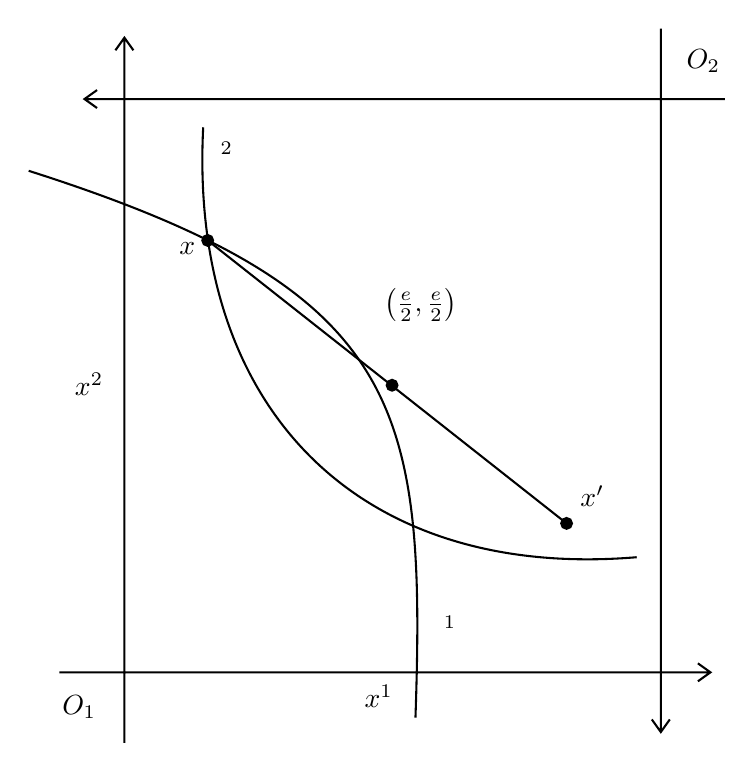
\begin{tikzpicture}[x=0.65pt,y=0.65pt,yscale=-1,xscale=1]
                %uncomment if require: \path (0,498); %set diagram left start at 0, and has height of 498

                %Shape: Axis 2D [id:dp15431277659194387] 
                \draw  (140,399.8) -- (502,399.8)(176.2,47) -- (176.2,439) (495,394.8) -- (502,399.8) -- (495,404.8) (171.2,54) -- (176.2,47) -- (181.2,54)  ;
                %Shape: Axis 2D [id:dp48430161652459225] 
                \draw  (510,81.1) -- (154,81.1)(474.4,433) -- (474.4,42) (161,86.1) -- (154,81.1) -- (161,76.1) (479.4,426) -- (474.4,433) -- (469.4,426)  ;
                %Curve Lines [id:da9749178354884357] 
                \draw    (220,96.8) .. controls (212,252.8) and (306,348.8) .. (461,335.8) ;
                %Curve Lines [id:da46802741379550783] 
                \draw    (123,121) .. controls (330,187) and (344,249) .. (338,425) ;
                %Shape: Circle [id:dp08891042852606446] 
                \draw  [fill={rgb, 255:red, 0; green, 0; blue, 0 }  ,fill opacity=1 ] (219.5,159.7) .. controls (219.5,158.04) and (220.84,156.7) .. (222.5,156.7) .. controls (224.16,156.7) and (225.5,158.04) .. (225.5,159.7) .. controls (225.5,161.36) and (224.16,162.7) .. (222.5,162.7) .. controls (220.84,162.7) and (219.5,161.36) .. (219.5,159.7) -- cycle ;
                %Straight Lines [id:da9146536136560517] 
                \draw    (222.5,159.7) -- (422,317) ;
                %Shape: Circle [id:dp04846876280996182] 
                \draw  [fill={rgb, 255:red, 0; green, 0; blue, 0 }  ,fill opacity=1 ] (322,240.2) .. controls (322,238.54) and (323.34,237.2) .. (325,237.2) .. controls (326.66,237.2) and (328,238.54) .. (328,240.2) .. controls (328,241.86) and (326.66,243.2) .. (325,243.2) .. controls (323.34,243.2) and (322,241.86) .. (322,240.2) -- cycle ;
                %Shape: Circle [id:dp03513551108035817] 
                \draw  [fill={rgb, 255:red, 0; green, 0; blue, 0 }  ,fill opacity=1 ] (419,317) .. controls (419,315.34) and (420.34,314) .. (422,314) .. controls (423.66,314) and (425,315.34) .. (425,317) .. controls (425,318.66) and (423.66,320) .. (422,320) .. controls (420.34,320) and (419,318.66) .. (419,317) -- cycle ;

                % Text Node
                \draw (140,410.8) node [anchor=north west][inner sep=0.75pt]    {$O_{1}$};
                % Text Node
                \draw (487,51.8) node [anchor=north west][inner sep=0.75pt]    {$O_{2}$};
                % Text Node
                \draw (308,405.2) node [anchor=north west][inner sep=0.75pt]    {$x^{1}$};
                % Text Node
                \draw (147,231.6) node [anchor=north west][inner sep=0.75pt]    {$x^{2}$};
                % Text Node
                \draw (352,366.6) node [anchor=north west][inner sep=0.75pt]    {$\succsim_{1}$};
                % Text Node
                \draw (228,103.2) node [anchor=north west][inner sep=0.75pt]    {$\succsim_{2}$};
                % Text Node
                \draw (205,159) node [anchor=north west][inner sep=0.75pt]    {$x$};
                % Text Node
                \draw (319,184.4) node [anchor=north west][inner sep=0.75pt]    {$\left(\frac{e}{2} ,\frac{e}{2}\right)$};
                % Text Node
                \draw (428,294.4) node [anchor=north west][inner sep=0.75pt]    {$x'$};
            \end{tikzpicture}
            \caption{Graphical test for envy-freeness.}
            \label{fig:L6-edgeworth-envy}
        \end{center}
    \end{figure}

\end{exercise}

\bibliographystyle{apacite}  % or another  style
\bibliography{references} % .bib file goes in ./bib/